\documentclass[a4paper,11pt]{article}
\usepackage[a4paper, includefoot,margin=1.5cm]{geometry}
\usepackage[parfill]{parskip}
\usepackage{ctable}
\usepackage{url}
\usepackage{graphicx}
\usepackage{paralist}
\usepackage{verbatim}

\begin{document}
\title{WebApps Group Project: Project Report} \date{12th June
  2013} \author{
  Thai Tam Nguyen $<$ttn211@imperial.ac.uk$>$\\
  Jo Schlemper $<$js3611@imperial.ac.uk$>$\\
  Terence Tse  $<$tt1611@imperial.ac.uk$>$ }
\maketitle
%\newpage

\section*{Introduction }

     The main focus of our application is to allow users  keep track of money that is owed to them by their friends or, indeed, how much they owe them. Originally inspired by such problems arising amongst flatmates and friends at university, we wanted to broaden the scope of potential users of our app. In addition to this, additional features he had in mind were, a messaging system, "wishlists" and shared calendars.
\\
\\     Our minimum requirement was to fulfil and provide the debt tracking functionality, offering a comprehensive visual feedback to the user. The other main requirement was to complete the messaging feature of the application as it enhances the applications overall usability - communication is key when dealing with money and we didn't want the user to have to delegate to a separate messaging application.
\\
\\     We also set secondary targets, most of which were just about completing the embellishing features, i.e. the "wishlists" and the calendar. Other targets we set for ourselves included personalised user profiles, which could be changed in the app settings, as well as making the app include solutions to common problems users would face (i.e. our equal split function for a transaction total). 



\section*{Project Management}
\subsection*{Group Structure}
In order to implement our application efficiently, we split the work between the team members, lead by our "captain" Jo Schlemper, who overlooked the overall progress of the project. \\
Terence worked mainly on the database, its state and maintenance. He was also concerned on writing the server side of the interactions between the database and the application itself.
Thai Tam worked mainly on the graphics of the application, including its scaling on multiple screens, and its user-friendliness aspects, and helped with the implementation of operations to be executed after user input.
Jo concerned himself with the interactions between the database and the application, as well as the operations resulting from user input and the client side operations. Being the leader of the group, he overlooked the work in general, and was key to bringing all parts of the application together.
 
\subsection*{Implementation Language}
We have chosen to develop an application for Android devices, including tablets such as the Nexus7, as they are becoming more commonly used. It is easy to spot someone in public transport, playing with their phone or other device.  \\
The Java IDE platform for Android development includes many useful libraries and templates, which render making basic graphics for an android application very easy. This means that it would be possible to implement interactions between the graphic elements of the application and the database early in our design, while still being able to ameliorate the visual aspects of the application some time later. Furthermore, the resources on Java based android developing are far more abundant and consistent than on any other language – this was very helpful in manipulating code.\\
\\
Another reason why we chose to develop on Android is because of the language feature. Android allows us to construct the view using XML files, which in terms of MVC design principle, enables us to separate the view from the rest by default. Another advantage is the Java is an object orientated language. This enables us to handle bunch of data easily and pass it around to different components of the program in the form of objects. Java also allows us to encapsulate the data, which is also advantageous in term of security. With the aforementioned features in mind, we chose Java as our implementation language

\subsubsection*{Server}
We have chosen Tomcat as a server, as it is the most extensively application server used in the world, and allows easy build and check of connected applications, especially when working with Java and its associated JREs.
Furthermore, it offers some kind of flexibility, as Tomcat is part of the Apache Jakarta Project - it is possible to run Apache on a server, but use Tomcat on another machine. This would be useful if we were to grow our project, or if we wanted to offer a high level of security and stability.

\subsubsection*{Database}
We have chosen to work with a PostgreSQL database as it is a very reliable and robust system. It is also compatible with a large range of platforms, including Windows and Unix, making it easy to work with and extend.
With this relational database, it was easy to express column dependencies between tables and the maintenance of the database was easy too. PostgreSQL is also heavily documented online which helped our group to learn how to use it. PostgreSQL had several nice features, e.g. allowing composite keys, constraints and default values for columns and sequences (generating a pseudo-unique id counter). These came in useful as when manually entering data we did not have to enter an id nor check for the next unique one. Lastly, the error messages are more useful and informative than for instance MySQL.

\begin{figure}[ht]
\begin{center}
\advance\leftskip-3cm
\advance\rightskip-3cm
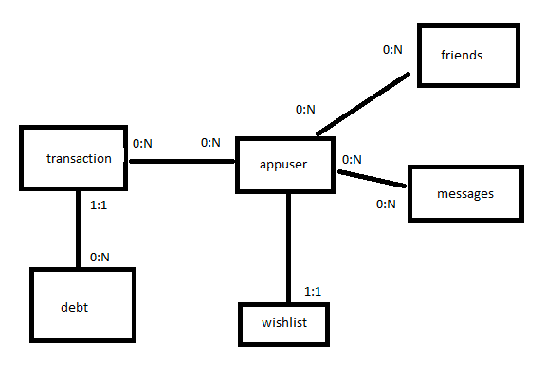
\includegraphics[keepaspectratio=true,scale=0.5]{uml}
\caption{Database UML}
\label{visina8}
\end{center}
\end{figure}

\subsection*{Design Process}
\subsubsection*{Planning}
As members of society, we feel a need to interact with one another, sometimes leading to requests. A common request, especially amongst friends, is “Could you please lend me x pounds?”, thus leading to debts. However, tracking the amount of money your friends owe you, as well as the amount you owe them can become a very cumbersome task. In order to resolve this problem, we have decided to create a system that would allow some user to track their debts easily. \\ \\
Our society is brimming with mobile devices – smart phones, tablets etc. are more prominent nowadays. As such, we have decided that developing an application for a mobile device would be a nice choice. However, each individual has different views of what to consider “ideal”. We therefore had to spend time studying and revising the content and layout of our application: should we include a full-fledged instant messaging system? Will the users need it? What problems will out users face which we can also help solve? After asking ourselves these questions, we have concluded that our application would include the following features: a transaction tracking system that would include the setting of new transactions, a calendar that would allow transaction deadlines, an instant messaging system, a synchronised wish list, user profiles, as well as a settings button that would enable the user to switch between two kinds of debt views; per person or per item. We then sketched by hand the main activities’ screen so everyone would have a concrete idea of what would be included in each one of the features available in our application and how we'd transition to different parts of the app such as from sign in, what messages should the user be shown and from transactions, what do they want to know about the transaction as well as placement of data.

\subsubsection*{Implementation and Testing}
We began implementation concurrently. We had planned thoroughly the whole system and so could split it into parts. Setting up the database and the server was done in parallel with designing the views and the basic graphics for our app's features. This followed an MVC approach, where we could separately design the view and the model which we then linked with the "control" later; our control were servlets which we implemented towards to mid-end of the project to link what we had already designed. We populated the database with dummies in order to test the correctness of our application. We meanwhile also ameliorated the graphics of the activity, scaling it, at first, for Nexus7 tablet screen size. We then repeated this cycle over all the relevant features of our app. We tested our app by inputting data as if in a real life transaction scenario and checked all the functionality in the same way.


\subsection*{Back-ups}
We have used Git as our version control for the whole duration of our project, and set up the repository on GitHub. This has allowed us to work in parallel, easily compare different versions of our project, as well as come back to a previous one if necessary. 


\section*{Program }
\subsection*{Description}
Our final product is an android application which keeps track of debts. Once a user registers to the database, the user can create a new transaction, view transactions and make a payment or a partial payment for the transactions. The application provides the ability to make transactions to an individual or a group. It also supports messaging for individuals or a group, which can be used as a mean to communicate with each other, urge one another to pay and so on. The view of the transactions can be customised according to the users’ preference: per person or per item. Per person displays a list of people who you owe or who owes you and total amount of the debt. Clicking on the entry allows you to view a profile page, from which you can nudge, message, call and make a new transaction to the person. It also provides a log of transactions you have with the person. Per transaction view gives you the name of the transactions instead of the people you owe. Both views are consistent in terms of data of course, they are merely different representations, linking to multiple views from the MVC pattern.

\begin{figure}[ht]
\begin{center}
\advance\leftskip-3cm
\advance\rightskip-3cm
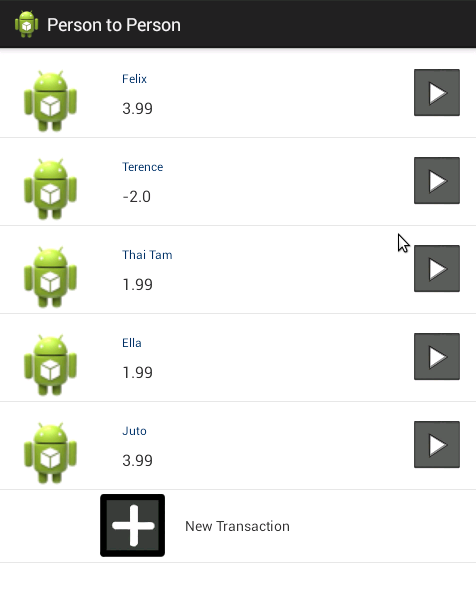
\includegraphics[keepaspectratio=true,scale=0.5]{perPerson}
\caption{Viewing bills per person}
\label{visina8}
\end{center}
\end{figure}

\begin{figure}[ht]
\begin{center}
\advance\leftskip-3cm
\advance\rightskip-3cm
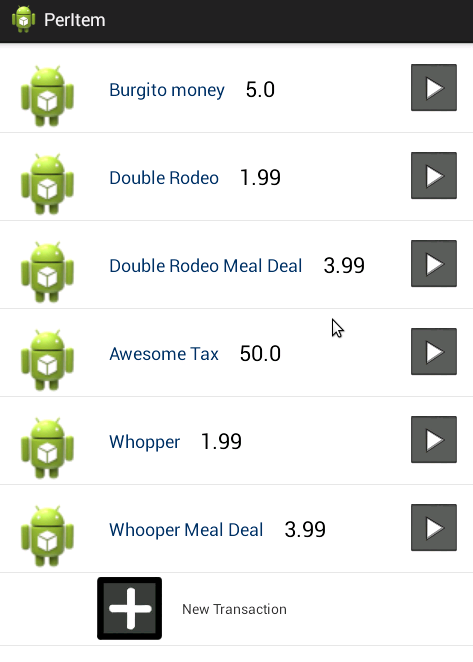
\includegraphics[keepaspectratio=true,scale=0.5]{perItem}
\caption{Viewing bills per item}
\label{visina8}
\end{center}
\end{figure}

\subsection*{Design Patterns}
Although the fundamental idea of the application is fairly simple, achieving the functionalities require careful considerations of design patterns. 

\subsubsection*{Classic 3-tier architecture}
For multiple users to interact with one another, it was necessary to have a convention for the communication of data. To achieve this we decided to deploy a classic 3-tier architecture as having a database on the server simplifies this communication process. Every time when a user requests to view or create transactions, the requests will be sent to the server through HTTP methods, GET or POST. For our application, it is unnecessary to serve a page; instead, we pass around a data between the client and the server in JSON format. The reason why we chose JSON is because it is a recognised standard format for passing data across networks. It means that there are many third party libraries for encoding and decoding JSON string. For the client side, we used the standard library from Android to decode JSON string; on the server side, we wrote a code which builds a JSON string. 

\begin{figure}[ht]
\begin{center}
\advance\leftskip-3cm
\advance\rightskip-3cm
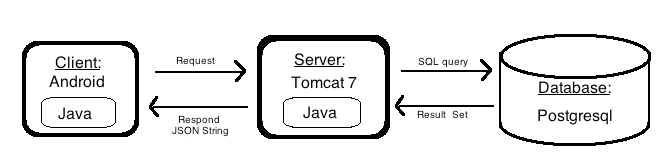
\includegraphics[keepaspectratio=true,scale=0.5]{3tier}
\caption{The 3-tier Architecutre}
\label{visina8}
\end{center}
\end{figure}

\subsubsection*{Builder pattern}
To build a JSON string from the server side, we wrote a class \texttt{JSONBuilder.java} which lets you to build a JSON string. A JSON string requires specific characters such as `$\lbrace$' `:' , alternatively writing the string manually could be erroneous so using the builder not only lets you make use of the pattern, it also simplifies the code and make it relatively easier to read. 

\begin{verbatim}
In JSONBuilder.java:
//... execute SQL query and obtain a set of results in transactionSet
// Build JSON string
JSONBuilder jb = new JSONBuilder();
jb.beginObject().append("returnCode",1).beginArray();
while (transactionSet.next()) {
//...Obtain the result
						
jb.beginObject().append("transid", transId)
                .append("name",transName)
                .append("total_amount",transAmount)
  .endObject();
}
jb.endArray().endObject();			
writer.println(jb.build());
\end{verbatim}

\subsubsection*{Singleton Pattern}

According to \texttt{apache.org}, it is recommended to have a single instance of a HttpClient per application. This is because instantiating a HttpClient is costly in resources. In our code, we decided to only instantiate a single instance of a HttpClient as we make a use of the client frequently. We don't want the client to take up all the resources. In \texttt{CustomHttpClient.java}, one can see that we have a static \texttt{getHttpClient()} method to get the single instance of it. The \texttt{getHttpClient()} is declared private because it will only be used in the static GET and POST methods defined in the class. All the other classes will use the methods defined here. 

\begin{verbatim}
In CustomHttpClient.java:
private static HttpClient getHttpClient() { //.... }

public static InputStream executeHttpPost(String url, 
List<NameValuePair> postParameters) throws Exception {
            HttpClient client = getHttpClient();
            //... make a request
}  
\end{verbatim} 

\subsubsection*{Concurrency}

Our program uses frequent network operations. However, these network operations could suffer from unpredictable delays, hence, we do not know exactly when the data arrives from the server. A thread executing the network operation needs to be blocked while waiting for the response from the server. In terms of the user experience, this is problematic because if the main thread executes the network operations, it could block itself until the response arrives. For android, the main thread is also responsible for generating user interacts and the views. Which implies that user will see your program freezing in every so often whenever the program performs network operations. In order to avoid this, we made heavy use of \texttt{AsyncTask} class. \texttt{AsyncTask} is an abstract class defined by Android and can be used to perform background operations on another thread, which in our case are network operations. By using this class, the user will not need to see the program "freezing"; instead, the view will be updated as the data arrives.     
  \begin{verbatim}
In MainActivity.java:
public void loginHandler(View view) {
    ...obtain data from user input

    // Ensure the network connection
    ConnectivityManager connMgr = (ConnectivityManager) 
    getSystemService(Context.CONNECTIVITY_SERVICE);
    if (ConnectionHelper.checkNetworkConnection(connMgr))
    //Create a new asynchronous task to verify the password from the server
        new PasswordVerifier().execute(phoneNo, password);
    else
        errorView.setText("No network connection");
}

private class PasswordVerifier extends AsyncTask<String,Void,Boolean>{
...
}
 \end{verbatim}
 
\subsubsection*{Observer Pattern}

All the GUI components for android follows the observer pattern. All the GUI components are subscribed for an event. When a user interacts (e.g. click) with the component an event will be created. The components by default do nothing but we can specify the behaviour by overriding the methods such as "onClickListener", or calling them from the XML using "android:onClick". For example, on our "transaction" window, the user can see a list of people who he or she owes to know how much one owes to different people.  

\begin{center}
\begin{verbatim}
In PerPeron.java:
	transList = (ListView) findViewById(R.id.PerPersonList);
	transList.setOnItemClickListener(new OnItemClickListener() {
		@Override
		public void onItemClick(AdapterView<?> a, View v, int pos, long id) {
			...
		}
\end{verbatim}
\end{center}

\begin{figure}[ht]
\begin{center}
\advance\leftskip-3cm
\advance\rightskip-3cm
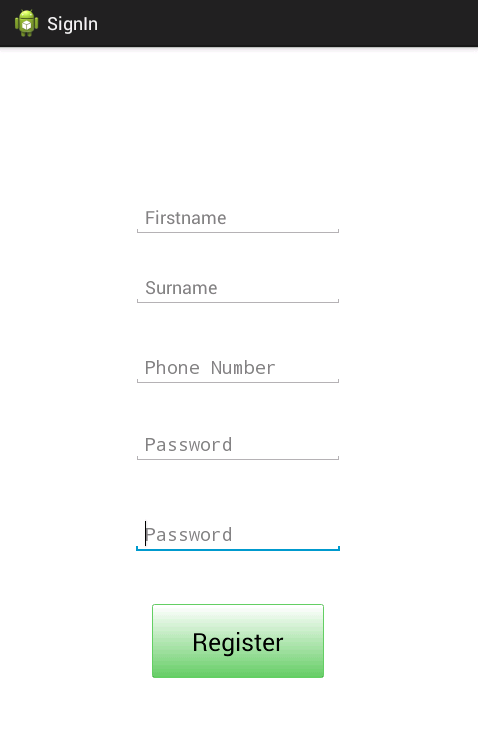
\includegraphics[keepaspectratio=true,scale=0.5]{signIn}
\caption{Sign in activity. The data will be sent as POST}
\label{visina8}
\end{center}
\end{figure}

\subsubsection*{Template Method}
Our program uses adapters in order to display the different transactions in two ways: per item and per person. However, these two modes essentially encapture the same behaviour: they display the amount that the user owes or is owed on the screen, and allows them to look into the details of each transaction. As such, we have implemented a template: 
\begin{verbatim}
public abstract class CustomAdapter<T> 
\end{verbatim}.
This class is extended by the PerPersonAdapter and the PerItemAdapter.

\subsubsection*{General Style}
In general, we tried to follow the basic design principle as much as possible, such as SOLID. Each classes has a single responsibility to one activity. Common methods such as Http methods are extracted out in a specific class. The project is "Open" to adding new features as this would only require adding new classes representing new activity or a process. In our project, we have a class which represents the data of transaction: \texttt{TransactionDetail.java}. We have considered encapsulation the fields in the class. We were required to pass data in \texttt{TransactionDetail} to different classes; for this, we used \texttt{Intent}, which is a class defined by Android. When passing data between different activities, one can put data into Intent on one side, retrieve data from Intent on the other side. This strategy respects the Law of Demeter; we do not need to know anything about the neighbours but simply know the "key" to retrieve the data we need. In this way we have achieved both good encapsulation and low coupling between different classes.
 
\section{Acknowledgement (doesn’t count, keep minimum)}

CustomHttpClient.java from Android Developers: http://developerrohit.blogspot.co.uk/2011/04/customhttpclientjava.html\\
Took as an inspiration for our client side HTTP methods such as GET and POST.

\subsection*{Copyright}
The images and icons we have used have all been created by our group, and therefore, we should not have any third-party copyright issue in those regards.
Some of our code used template code provided by Android Developers when downloading the Android SDK. As such, it is not subject to copyright issues. Furthermore, little "skill and labour" were used in the process of using these templates, and their usage is therefore not liable for pursuit. In addition, the use of available libraries is not to be considered as stealing, although the libraries themselves may be licensed.\\
\\However, if we were to commercialise the app, we would need to license all our work, including our database set up, in order for third parties not to steal our work. We would also need to get database rights in order to form a database of all users and their relevant informations, such as phone numbers, friend lists, etc. \\
Unless we wanted to let our application be open sourced, we would also need to remove, or hide our Git repository on GitHub. Otherwise, we would need to license our product with an open source license.

\section*{Conclusion}
Although we have reached the end of this project, there are several reflections we have to make about our progress and what we have to show. 
\\
\\Our app meets all of our main requirements. We have managed to implement both the transaction logs and the messaging system within the app. Our transaction log is able to be viewed in two modes, per person and per transaction and the user may make additions and adjustments to transactions. The app clearly displays the transactions in chronological order whilst in per transaction mode and allows the user to view detailed information about the transaction easily. Whilst in per item mode, our app accurately displays the overall debt balance between the user and their friends, allowing a much more laid back and simplistic view on transactions between them.
\\
\\We have additionally managed to reach a couple of our targets, including the two view mode mentioned above, and the "wishlist", the neat feature of being able to place all your desired items onto a shared list so your friends may buy them if they are in the vicinity of a supermarket. We included the equal split button while adding a new transaction, another handy tool we thought our app should offer. We've managed to also add in reminders, preset messages for users to send to those friends who aren't quite so prompt with their payments, via the messaging system.
\\
\\Unfortunately, some of our targets have not been managed to be met. Our main regret is not being able to fully implement the shared Calendar feature our group envisioned. Though it is indeed a loss, it does not exactly detract from the main functionality of the app and can be substituted for something more tangible in real life; for example, an actual calendar, though at the expense of paper!
\\
\\Our other main regret was that we were unable to add personalised views to the settings of the app. It renders the user unable to customise the look of the application in their taste. 
\\
\\
We envisioned our app to be simple and easy to use, as a result we fell into the trap of also envisioning the implementation to not be so difficult, as a result. This was not the case. Getting to grips with new and unfamiliar development tools consumed a lot of time. There was a lot of frustration with how unintuitive it was to design the GUI of the app via the android developer toolkit.
\\
\\ We learnt that there are any things to consider when designing such a simple app and should definitely not underestimate the workload in the future. 
From this project we have definitely gained a lot of useful skills. Designing for an android app has taught us a lot about making a web based application. We can also take away the ability to work with a server and integrate a database into such an application. Learning PSQL was also beneficial to our skillset and should come in handy in the future; 
\\
\\In the future, we would definitely improve our time management on such a task. We had underestimated the amount of work and thought that actually would go into integrating a database into a web application, all of which we had little to no prior experience.
This way, we would have had more time to complete the targets that we had set at the beginning and maybe even extend the app further.
\\
\\ 
We'd also spend a lot more time in the design and overall flow of the application or whatever similar task we decide to embark on in the future. There were time in this project where specific implementations of app features that we had mixed opinions about and sometimes were unclear ofwhat we all wanted it to be like in the final version.


\end{document}
